%15_adverserial_search.tex
%notes for the course COMS10007 taught at the University of Bristol
%Conor Houghton conor.houghton@bristol.ac.uk

%To the extent possible under law, the author has dedicated all copyright 
%and related and neighboring rights to these notes to the public domain 
%worldwide. These notes are distributed without any warranty. 

\documentclass[11pt,a4paper]{scrartcl}
\typearea{12}
\usepackage{graphicx}
\usepackage{pstricks}
\usepackage{listings}
\usepackage{tikz-qtree}
\lstset{language=C}
\usepackage{fancyhdr}
\pagestyle{fancy}
\lfoot{\texttt{github.com/conorhoughton/COMS10007}}
\cfoot{}
\rhead{\thepage}
\lhead{COMS10007 - algorithms 15\_adversarial\_search (q) - Conor}

\begin{document}

\section*{15 - adversarial search}

Here we will consider adversarial search: algorithms designed to allow
a computer to develop an optimal strategy for an adversarial game, or
a process that can be rephrased as a game. In particular we will
consider the minimax algorithm, a na\"ive AI which has been useful; it
is na\"{i}ve in the sense that it does not perform sophisticated
pattern recognition using modern biometic neural networks like
deep-learning networks, instead it relies on the brutish computational
power of a computer to \lq{}play ahead\rq{} and see the consequence of
different moves. With tweaks, this is the algorithm that allowed Deep
Blue to beat Garry Kasparov, the world chess champion, in 1997,
realizing a proposal, originally due to Claude Shannon, that computers
can play chess. It is not the algorithm that allowed AlphaGo to beat
Lee Sidol, a 9th Dan Go champion, in 2016, that was a deep learning
network.

Roughly speaking we are thinking about a game without chance where two
players alternate in taking a move which changes the game state. In
chess the game state is the position of the pieces on the board, in go
the position of the stones, in tic-tac-toe the number and position of
the Xs and Os on the grid. In adverserial search a tree is constructed
with the current state of the game as the root: the nodes will be game
states and the different edges from a node will correspond to
different possible moves. At first the leaves, the terminal nodes,
correspond to final game states, which will be a win for one or other
player or a draw. The overall strategy is to score the leaves and to
propagate those scores upwards under the assumption that each player
plays optimally. It is easiest to describe this through an example. 

\subsubsection*{Nim example}

Nim is a simple game using counters for two players; the counters are
divided into some number of piles and the players take turns removing
counters. In their turn a player must take at least one counter and can take
as many counters as they like, provided they only come from one
pile. Thus, in each turn each player removes counters from only one
pile. The winner is the player who takes the last piece. An example
game is given in Table~\ref{tab:nim_example}

\begin{table}
\begin{tabular}{cccc|l}
5&2&6&3&Initial arrangement\\
1&2&6&3&\textbf{A}oife takes four from pile one\\
1&2&6&0&\textbf{B}rendan takes three from pile four\\
1&2&1&0&\textbf{A}oife takes five from pile three\\
1&1&1&0&\textbf{B}rendan takes one from pile two\\
1&0&1&0&\textbf{A}oife takes one from pile two\\
1&0&0&0&\textbf{B}rendan takes one from pile two\\
0&0&0&0&\textbf{A}oife takes one from pile one and wins
\end{tabular}
\caption{An example of two players playing nim; this illustrates game play, neither player is playing optimally. The four columns give the number of counters in the four piles directly after the move described in the same row.\label{tab:nim_example}}
\end{table}

Nim can be enjoyable to play, but it is mostly beloved of
mathematicians and computer scientists because it is a good example to
use in explanations like this one and because it was solved as a game,
for all numbers of piles and counters, in 1902 by Charles L. Bouton,
in a paper which is considered to have founded combinatorial game
theory. What we are interested in here stops short of solving the game
analytically, instead in Fig.~\ref{fig:nim} we map out a tree giving
all possible moves for nim with three piles of two. Thus, from the
initial configuration $(2,2,2)$ leaving out alternatives that are
equivalent to each other, there are two possible moves, the player can
take one or two counters from one of the piles, leading to $(1,2,2)$
or $(0,2,2)$. From $(1,2,2)$ there are then three alternatives,
leading to $(0,1,2)$, $(1,1,2)$ and $(0,2,2)$, and so on.

Now the leaves of the tree all have two zeros, whoever has the next
move wins. This means we can score the leaves; for definiteness let's
imagine Aoife has the first go so if this is to be an AI for a
computer then Aoife is the computer and the purpose of this
calculation is to choose which move Aoife should make at $(2,2,2)$ to
win. Obviously the different levels in the tree alternate between the
two players, so the level of the root corresponds to Aoife moving, the
next level, with $(1,2,2)$ and $(0,2,2)$ to Brendan and so on. The
different levels are sometimes called \textsl{ply} in this context.

\begin{figure}
\begin{center}
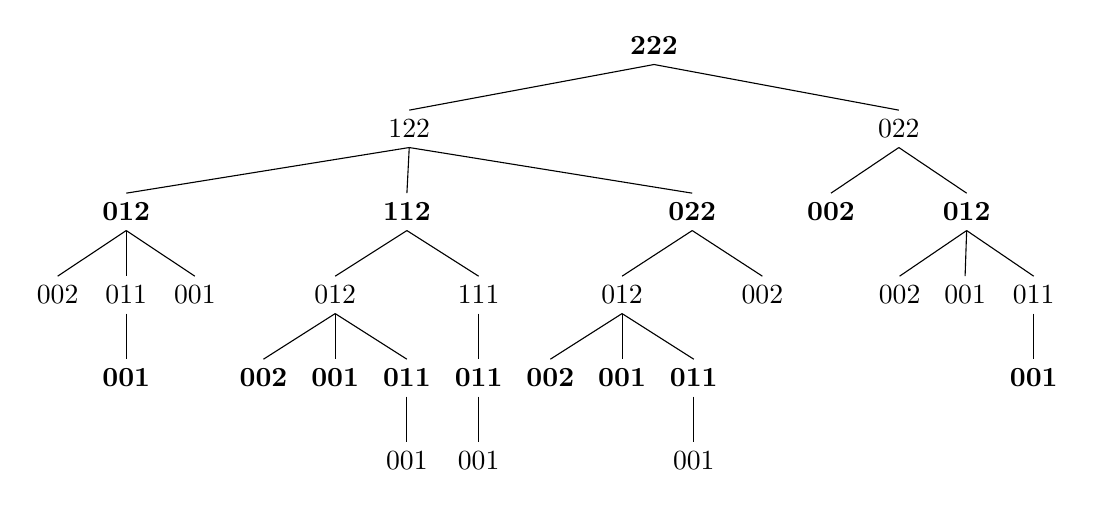
\begin{tikzpicture}
\Tree
[.\textbf{222}   
  [.122
    [.\textbf{012} 
      [.002 ]
      [.011 \textbf{001} ]
      [.001 ]
    ]
    [.\textbf{112} 
      [.012
        [.\textbf{002} ]
        [.\textbf{001} ]
        [.\textbf{011} 001 ]
      ]
      [.111
        [.\textbf{011} 001 ]
      ]
    ]
    [.\textbf{022} 
      [.012
        [.\textbf{002} ]
        [.\textbf{001} ]
        [.\textbf{011} 001 ]
      ]
      [.002 ]
    ]
  ]
  [.022
    [.\textbf{002} ]
    [.\textbf{012} 
      [.002 ]
      [.001 ]
      [.011 \textbf{001} ]
    ]
  ]
]
\end{tikzpicture}
\end{center}
\caption{The whole game tree for nim starting with $(2,2,2)$; some
  equivalent choices have been left out, so it includes $(1,2,2)$ on
  the second ply, but not $(2,1,2)$; for clarity the triples are
  arranges in ascending order. Alternative ply are bolded to help keep
  track of who is playing, Aoife is bold, whereas her opponent is
  unbolded, so for a bolded node Aoife takes the next
  move. \label{fig:nim}}
\end{figure}


We will score +1 for leaves where Aoife has the next go and is thus
able to win, -1 if Brendan does. This is shown in
Fig.~\ref{fig:nim-leaves}; the problem is that the leaves are far
removed from the current move, Aoife is at $(2,2,2)$ and decided
between $(1,2,2)$ and $(0,2,2)$; we need to move the scoring up from
the leaves to the root.

\begin{figure}
\begin{center}
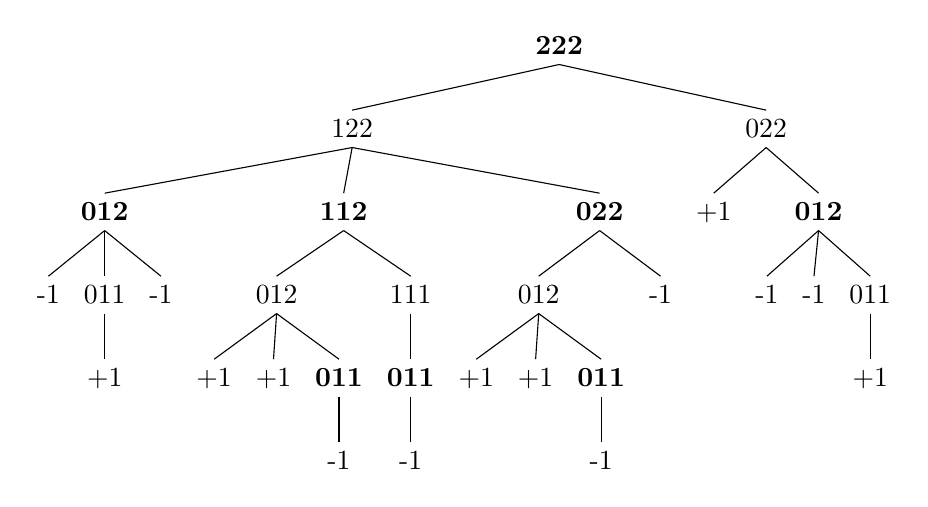
\begin{tikzpicture}
\Tree
[.\textbf{222}   
  [.122
    [.\textbf{012} 
      [.-1 ]
      [.011 +1 ]
      [.-1 ]
    ]
    [.\textbf{112} 
      [.012
        [.+1 ]
        [.+1 ]
        [.\textbf{011} -1 ]
      ]
      [.111
        [.\textbf{011} -1 ]
      ]
    ]
    [.\textbf{022} 
      [.012
        [.+1 ]
        [.+1 ]
        [.\textbf{011} -1 ]
      ]
      [.-1 ]
    ]
  ]
  [.022
    [.+1 ]
    [.\textbf{012} 
      [.-1 ]
      [.-1 ]
      [.011 +1 ]
    ]
  ]
]
\end{tikzpicture}
\end{center}
\caption{Here the leaves have been scored, +1 for a win for Aoife, -1
  if Brendan wins. Since each player takes just one move in each turn,
  it is easy to score the leaves, the bold ones go to +1, the unbolded
  to -1.\label{fig:nim-leaves}}
\end{figure}

In Fig.~\ref{fig:nim-leaves_1} the scoring has been moved upwards in a
simple way, since the only legal moves from $(0,1,1)$ lead to
$(0,0,1)$ or equivalently $(0,1,0)$ this means $(0,1,1)$ leads to the
same result as $(0,0,1)$ and so the score from the leaf is moved up
one. 

However this reasoning isn't enough if a node has more than one leaf,
as for example is the case for 012:a in
Fig.~\ref{fig:nim-leaves_1}. Here minimax search uses the
assumption that each player is playing optimally, so Aoife makes the
choice that maximizes the score, and Brendan the choice that minimizes
it. In the case of 012:a, it is Brendan's turn so he will choose the
move that will give the lowest of the three scores on offer, that is
the one that gives -1, hence this node is also worth -1; similarly for
\textbf{012}:b it is Aoife's go so she will choose the move that gives
+1. This assumption allows the scores to be propagated upwards, with
each time the parent inheriting either the lowest or highest of the
scores of its children, depending on whose go it corresponds to. 

\begin{figure}
\begin{center}
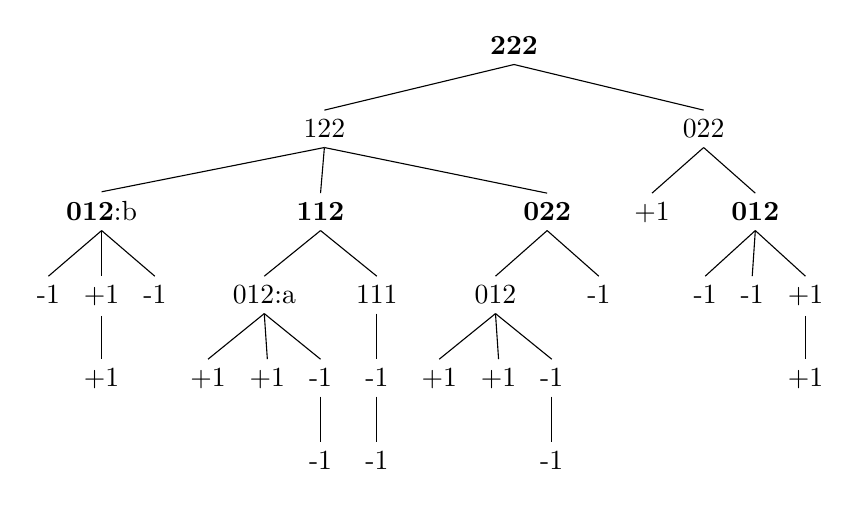
\begin{tikzpicture}
\Tree
[.\textbf{222}   
  [.122
    [.\textbf{012}:b 
      [.-1 ]
      [.+1 +1 ]
      [.-1 ]
    ]
    [.\textbf{112} 
      [.012:a
        [.+1 ]
        [.+1 ]
        [.-1 -1 ]
      ]
      [.111
        [.-1 -1 ]
      ]
    ]
    [.\textbf{022} 
      [.012
        [.+1 ]
        [.+1 ]
        [.-1 -1 ]
      ]
      [.-1 ]
    ]
  ]
  [.022
    [.+1 ]
    [.\textbf{012} 
      [.-1 ]
      [.-1 ]
      [.+1 +1 ]
    ]
  ]
]
\end{tikzpicture}
\end{center}
\caption{Here the score of the leaves with no siblings have been moved
  up to their parent. Two of the nodes have been labelled with letters
  012:a and \textbf{012}:b, these letters are just to help refer to
  the nodes in the text and have no meaning in the context of the
  game. \label{fig:nim-leaves_1}}
\end{figure}


The first step for this process is shown in
Fig.~\ref{fig:nim-leaves_2}; notices that in the case of
\textbf{112}:a the two children each have score -1 so although this is
Aoife's turn, she is forced to choose a losing move and \textbf{112}:a
is scored -1. Finally in Fig.~\ref{fig:nim-leaves_3} the scores have
propagated to the top and we see that if Aoife takes the right option,
$(0,2,2)$, she will win no matter what Brendan does, whereas if she
takes the left option Brendan can win if he plays optimally.


\begin{figure}
\begin{center}
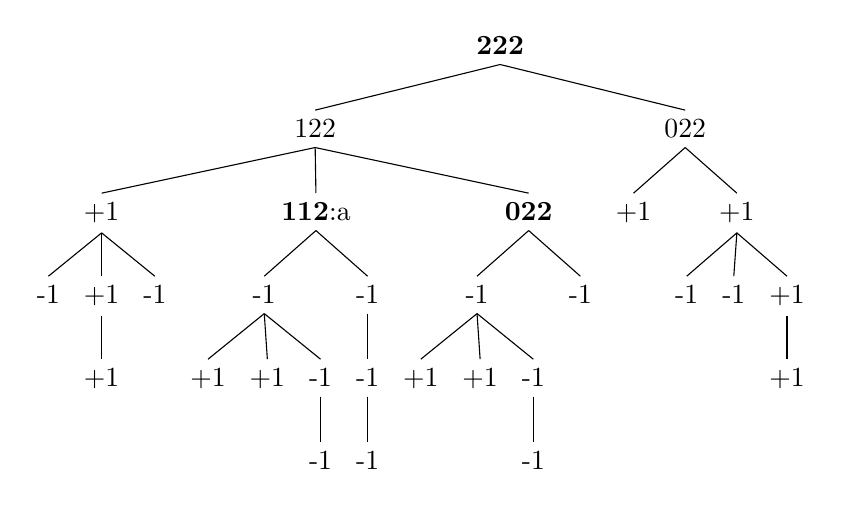
\begin{tikzpicture}
\Tree
[.\textbf{222}   
  [.122
    [.+1 
      [.-1 ]
      [.+1 +1 ]
      [.-1 ]
    ]
    [.\textbf{112}:a 
      [.-1
        [.+1 ]
        [.+1 ]
        [.-1 -1 ]
      ]
      [.-1
        [.-1 -1 ]
      ]
    ]
    [.\textbf{022} 
      [.-1
        [.+1 ]
        [.+1 ]
        [.-1 -1 ]
      ]
      [.-1 ]
    ]
  ]
  [.022
    [.+1 ]
    [.+1 
      [.-1 ]
      [.-1 ]
      [.+1 +1 ]
    ]
  ]
]
\end{tikzpicture}
\end{center}
\caption{Some of the scores have been propogated upwards, this process now propagates until the current decision point is reached. Again, the label \textbf{112}:a has no meaning in the game context but is there to help discussion in the text. \label{fig:nim-leaves_2}}
\end{figure}


\begin{figure}
\begin{center}
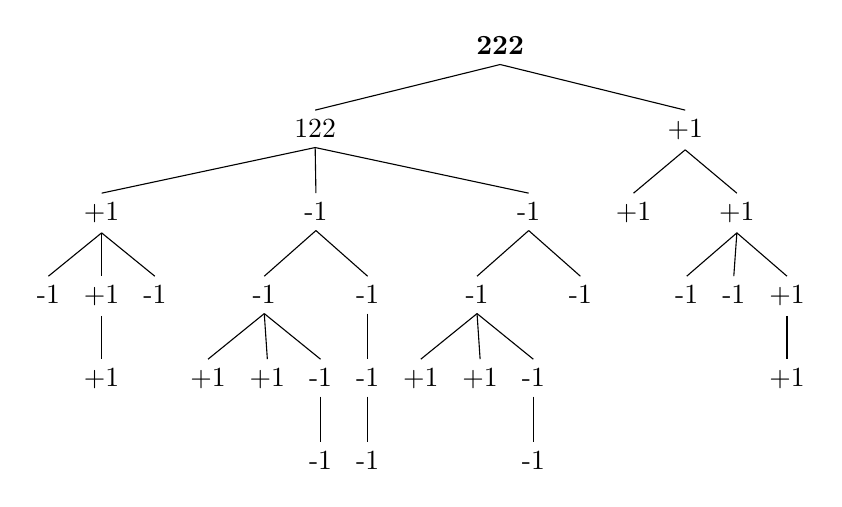
\begin{tikzpicture}
\Tree
[.\textbf{222}   
  [.122
    [.+1 
      [.-1 ]
      [.+1 +1 ]
      [.-1 ]
    ]
    [.-1
      [.-1
        [.+1 ]
        [.+1 ]
        [.-1 -1 ]
      ]
      [.-1
        [.-1 -1 ]
      ]
    ]
    [.-1 
      [.-1
        [.+1 ]
        [.+1 ]
        [.-1 -1 ]
      ]
      [.-1 ]
    ]
  ]
  [.+1
    [.+1 ]
    [.+1 
      [.-1 ]
      [.-1 ]
      [.+1 +1 ]
    ]
  ]
]
\end{tikzpicture}
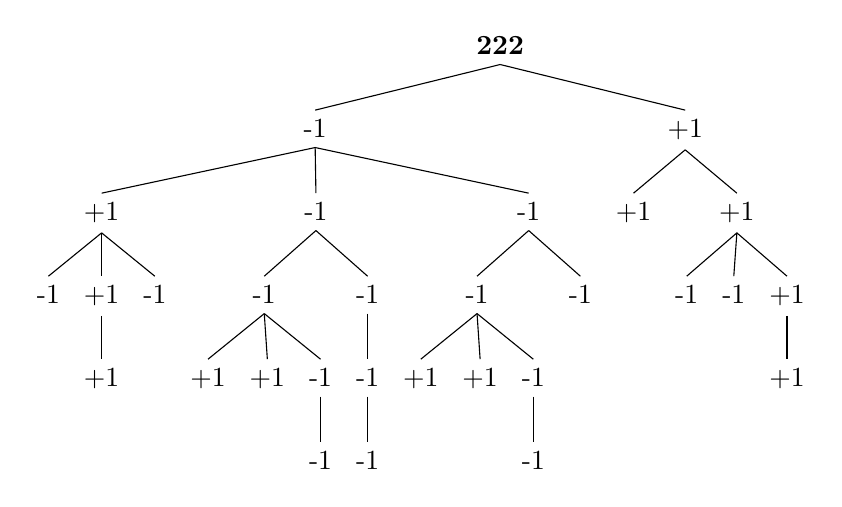
\begin{tikzpicture}
\Tree
[.\textbf{222}   
  [.-1
    [.+1 
      [.-1 ]
      [.+1 +1 ]
      [.-1 ]
    ]
    [.-1
      [.-1
        [.+1 ]
        [.+1 ]
        [.-1 -1 ]
      ]
      [.-1
        [.-1 -1 ]
      ]
    ]
    [.-1 
      [.-1
        [.+1 ]
        [.+1 ]
        [.-1 -1 ]
      ]
      [.-1 ]
    ]
  ]
  [.+1
    [.+1 ]
    [.+1 
      [.-1 ]
      [.-1 ]
      [.+1 +1 ]
    ]
  ]
]
\end{tikzpicture}
\end{center}
\caption{The scores are propagated to the root showing that Aoife can either force a win or risk losing.\label{fig:nim-leaves_3}}
\end{figure}


\subsubsection*{Scoring}
Obviously one disadvantage of adverserial search is that it ignores
any psychology. Another obvious example game is tic-tac-toe,
tic-tac-toe is a silly game because, as we all know, optimal play
always leads to a draw and so adversial search will propagate a value
of 0 to the root; however, if for example playing against a child, it
might be worth playing to win on the assumption your opponent won't
play optimally; this would involve guessing which strategy is most
likely to trick them. However a bigger issue is the combinatorial
explosion implicit in most games; for (2,2,2) there is only a modest
number of valid moves at each level, a larger number of counters and
piles would obviously expand this, however this is still modest
compared to the number of choices for a game like chess or go.

In a chess game there are typically 37 available moves and a typical
chess game has 100 moves in total, clearly this makes exploring the
game to the end infeasible. In go the situation is even more extreme;
the number of possible moves is usually more than 100 and a game
usually involves more turns than chess. This creates a horizon, a
distance down the tree beyond which it is infeasible, given computer
speed and game tempo, to search which means that the leaves, the
terminal nodes, often don't represent a final resolution of the game
and so they can't be attributed a score to represent win, loss or
draw.

The way out of this is to score the leaves using a heuristic, some
machine-calculable number describing how good a given game
configuration is. In the case of chess, for example, Shannon's
original proposal was that each player was given a score based on
their remaining pieces, one point for each pawn, three for each knight
or bishop, five for a rook and nine for the queen, on their position,
so for example there is a half point taken off for each doubled pawn,
that is one pawn behind another and on their mobility, with 0.1 points
for each available move. In addition a checkmate had a value of 200 to
trump all other considerations. The score for the position is the
difference between the two players. Now, in this scheme, each leaf is
evaluated using the heuristic and the score is propagated backwards
under the assumption that each player plays optimally.

A sketch of a program implementing minimax is given in
Table~\ref{c_minimax}.
   
\begin{table}
\begin{lstlisting}[numbers=left]
int which_child(Node* a)
{
   max_value(a);
   return a.best_child;
}

float max_value(Node* a)
{
   if(terminal_node(a)) return utility(a);

   int i;
   float v=-big_number,u;
   
   for(i=0;i<number_of_children(a);i++){
      u=min_value(get_child(a,i));
      if(u>v){
         v=u;
         a->best_child=i;
      }
   }
   return v;
}

float min_value(Node* a)
{
   if(terminal_node(a)) return utility(a);

   int i;
   float v=big_number,u;
   
   for(i=0;i<number_of_children(a);i++){
      u=max_value(get_child(a,i));
      if(u<v){
         v=u;
         a->best_child=i;
      }
   }
   return v;
}
\end{lstlisting}
\caption{Minimax. This code implements the minimax algorithm
  recursively, the recursion alternates, with \texttt{max\_value}
  calling \texttt{min\_value} and visa versa. It is not full working
  code in the sense that it relies on a \texttt{Node} struct which is
  not given along with a number of functions: \texttt{terminal\_node}
  returns true for a leaf and false otherwise, \texttt{utility}
  returns the score, \texttt{number\_of\_children} returns the number
  of children and \texttt{get\_child} returns the \texttt{i}th
  child. It also has \texttt{best\_child} to keep track of the child
  with the optimal score.\label{c_minimax}}
\end{table}

In practice a poor chess player looks forward four ply; a great one
eight but a great player also has more global ideas and intuitions
about the game, basically their heuristic is better. The computer that
beat Kasparov could look forward roughly 12 ply, the extra four ply
allowed it to beat the human; however, Deep Blue also did pruning, it
didn't look down every branch. This is what we discuss next.

\subsubsection*{Alpha-beta pruning}

In practice this scheme is supplemented by lots of tricks, for a start
different scoring schemes could be experimented on, a \lq{}book\rq{}
of well known opening sequences and endgames could stored; even in the
mid-game a playbook of zingers could help with common plays. Often
\lq{}interesting\rq{} branches are explored deeper. Another, more concrete,
improvement is provided by pruning. This is easy to understand given
an example; first consider the simple example given by the portion of
the nim tree given in Fig.~\ref{fig:nim-alpha-beta}; imagine we are
trying to score the $(1,2,2)$ node as part of a larger evaluation. In
Fig.~\ref{fig:nim-alpha-beta}B we see that after the left-most branch
has been scored we have a score of -1, since here Brendan is to play
at $(1,2,2)$ and -1 is the best he can do, we don't need to evaluate
the other two branches, they cannot beat the -1 we already have. Of
course, this was partly a matter of luck, if we had done the rightmost
branch first it would have given a +1, and at least one more branch
needs to have been evaluated.

\begin{figure}
A)
\begin{center}
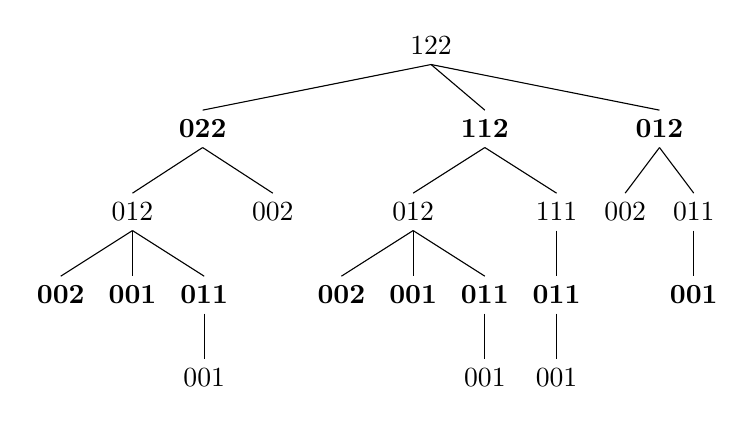
\begin{tikzpicture}
\Tree  
[.122
  [.\textbf{022} 
    [.012
      [.\textbf{002} ]
      [.\textbf{001} ]
      [.\textbf{011} 001 ]
    ]
    [.002 ]
  ]
  [.\textbf{112} 
    [.012
      [.\textbf{002} ]
      [.\textbf{001} ]
      [.\textbf{011} 001 ]
    ]
    [.111
      [.\textbf{011} 001 ]
    ]
  ]
  [.\textbf{012} 
    [.002 ]
    [.011 \textbf{001} ]
  ]
]
\end{tikzpicture}
\end{center}
B)
\begin{center}
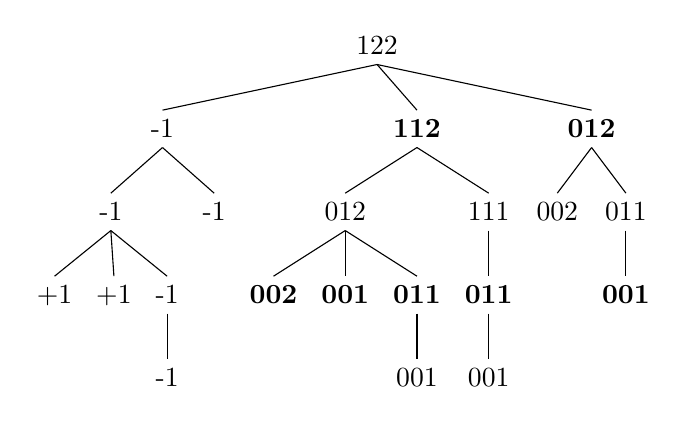
\begin{tikzpicture}
\Tree  
[.122
  [.-1
    [.-1
      [.+1 ]
      [.+1 ]
      [.-1 -1 ]
    ]
    [.-1 ]
  ]
  [.\textbf{112} 
    [.012
      [.\textbf{002} ]
      [.\textbf{001} ]
      [.\textbf{011} 001 ]
    ]
    [.111
      [.\textbf{011} 001 ]
    ]
  ]
  [.\textbf{012} 
    [.002 ]
    [.011 \textbf{001} ]
  ]
]
\end{tikzpicture}
\end{center}
\caption{A portion of the nim tree. In A) the whole tree is shown, in
  B) the left most branch has been score by propagating upwards from
  the leaves.\label{fig:nim-alpha-beta}}
\end{figure}

Alpha-beta pruning is a kind of second order version of
pruning. Consider the tree in Fig.~\ref{fig:partial}; in this tree the
aim is to get the score for the node labelled \lq{}unknown score
a\rq{}, in this example this node is the maximizing node. So far the
left sub-branch has been scored to give 20 but the right branch hasn't
been finished, in fact the first, leftmost, branch of the right branch
has been scored to give 10; now \lq{}unknown score b\rq{} is a
minimizing node, so although most of its children haven't been scored
we know that it will score no more than 10 because that score is
already available. Since \lq{}unknown score a\rq{} is a maximimizing
node it will never choose \lq{}unknown score b\rq{} since 20 is bigger
than 10. For this reason the other unscored children of \lq{}unknown
score b\rq{} don't need to be evaluated and this whole branch can be
pruned, freeing up more time to explore elsewhere. This is alpha-beta
pruning.

\begin{figure}
\begin{center}
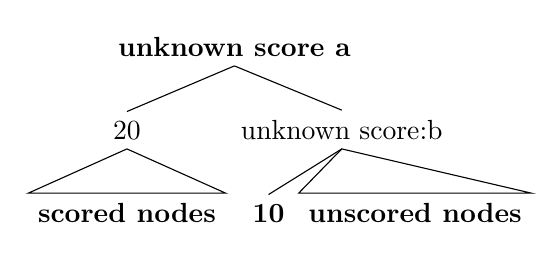
\begin{tikzpicture}
\Tree
[.\textbf{unknown~score~a}
  [.20 \edge[roof];{\textbf{scored nodes}} ]
  [\textbf{10} \edge[roof];{\textbf{unscored nodes}} ].unknown~score:b 
]
\end{tikzpicture}
\end{center}
\caption{Here the left branch has been fully scored, the right branch has only been partially scored, the left part gives 10, the rest hasn't been considered yet.\label{fig:partial}}
\end{figure}

Outline code for running minimax with alpha-beta pruning is given in
Table~\ref{c_alpha_beta}. This code might not seem completely
transparent at first since it is tricky to see how to keep track of
when to prune, to see how it works consider running it on the tree in
Fig.~\ref{fig:partial}. The root calls \texttt{max\_value} with
\texttt{below} set to $-\infty$, or equivalent, and \texttt{above} set
to $\infty$. The first node gives 20, so \texttt{below} is set to 20;
this means \texttt{min\_value} is called on the right branch with
\texttt{below} as 20; when the first branch returns 10 this is
compared to \texttt{below} and since $10<20$ this returns 10 and the
other nodes are not evaluated.

   
\begin{table}
\begin{lstlisting}[numbers=left]
int which_child(Node* a)
{
   max_value(a,-big_number,big_number);
   return a.best_child;
}

float max_value(Node* a,float below,float above)
{
   if(terminal_node(a)) return utility(a);

   int i;
   float v=big_number,u;
   
   for(i=0;i<number_of_children(a);i++){
      u=min_value(get_child(a,i),below,above);
      if(u>v){
         v=u;
         a->best_child=i;
      }
      if(v>=above) return v;
      if(v>below) below=v;
   }
   return v;
}

float min_value(Node* a)
{
   if(terminal_node(a)) return utility(a);

   int i;
   float v=-big_number,u;
   
   for(i=0;i<number_of_children(a);i++){
      u=max_value(get_child(a,i),below,above);
      if(u<v){
         v=u;
         a->best_child=i;
      }
      if(v<=below) return v;
      if(v<above) above=v;
   }
   return v;
}
\end{lstlisting}
\caption{Minimax with alpha-beta pruning. Here \texttt{above} and \texttt{below} ae used to keep track of pruning values; the clever thing is how the pruning values are pushed down from above.\label{c_alpha_beta}}
\end{table}



\end{document}
